
\chapter{Plenoptic De-blurring}
\label{chap:plenoptic_deblurring}

\section{Light Field Theory}
\label{sec:light_field_theory}

The light field is a mathematical description of the way light propagates.
Another name for this is the \enquote*{Plenoptic Function}, from the Latin \enquote*{plenus}, meaning full, and \enquote*{optic}, meaning light.
The plenoptic function describes every possible configuration a light ray could ever be in, encompassing the three spatial dimensions, two angular dimensions, temporal changes as well as frequency (colour), phase and polarisation changes.
In most computer vision literature the phase and polarisation elements are ignored, leading to a 7-dimensional definition of the plenoptic function;

\begin{equation}
\label{eq:plenoptic_function}
P = P(V_x, V_y, V_z, \theta, \phi, t, \lambda)
\end{equation}

\noindent
where $V_x$, $V_y$ and $V_z$ are the spatial dimensions, $\theta$ and $\phi$ are the angular dimensions, $t$ is the temporal dimension and $\lambda$ describes the colour of the ray. 

The plenoptic function in this form was first described by Adelson and Bergen in 1991 \cite{adelson1991plenoptic}.
Adelson and Bergen developed a light field theory by asking the fundamental question \enquote{What can be seen?} They stressed that the plenoptic function is the sole visual communication link between physical objects and the eye.
They also suggested that the function of \enquote*{early vision} in biological and artificial organisms is to sample the derivative of this function along various dimensions such as \enquote*{change in colour with x} or \enquote*{change in brightness with time}.

In computer vision literature, many different representations of the light field have been proposed, each emphasising different aspects of the plenoptic function.
McMillan and Bishop discuss the representation of 5D light field images ($V_x$, $V_y$, $V_z$, $\theta$ and $\phi$) as a set of multiple panoramic images taken at different physical locations \cite{mcmillan1995plenoptic}.
Importantly, in free-space (space free of occluding objects), one of the spatial dimensions is redundant, a consequence of the fact that radiance does not change along a line unless blocked \cite{levoy1996light}.
Thus, for free space, the 5th light field dimension can be dropped, giving a 4D light field definition.

Levoy and Hanrahan describe a parameterisation for the 4D light field which they term a \enquote*{light slab} \cite{levoy1996light}.
In this parameterisation, they describe a light ray by it's intersection through two arbitrarily placed planes in world space (Figure \ref{fig:light_slab}).

\begin{figure}[h]
\centering
\includegraphics[width=12cm]{light_slab.pdf}
\caption[The Light Slab Parameterisation of a 4D Light Field]{
The Light Slab Parameterisation of a 4D Light Field, described by Levoy and Hanrahan \cite{levoy1996light}.
A light ray is defined as passing through two arbitrary planes in world-space.
By their convention, both planes range from 0 to 1, and the dimensions are labeled $u$ and $v$, and $s$ and $t$ for the first and second planes respectively.
}
\label{fig:light_slab}
\end{figure}

The light slab parameterisation is useful as is similar to the design used in many modern light field cameras.
Traditional cameras generally sample the Light Field along two dimensions (x and y pixel locations) and in the colour dimension.
This is done using a 2D array of light-sensitive pixel elements, masked in a pattern to detect different light wavelengths (normally corresponding with the colours \enquote*{Red}, \enquote*{Green} and \enquote*{Blue}).
While there is active research in developing angle-sensitive pixels \cite{wang2009angle, wang2011angle, wang2012angle}, most modern light field cameras encode angular information by mapping ray angles to 2D sensor array locations, sacrificing spatial resolution for angular resolution.

Such cameras were first envisaged in 1996; independent research by Gortler et al. and Levoy et al. suggested it was possible to capture 4D light field information using a traditional camera sensor with some modifications \cite{gortler1996lumigraph, levoy1996light}.
Such a camera was physically constructed recently by Ren Ng and is described in his dissertation \cite{ng2006digital}.
Ng's prototype light field camera used a microlens array placed over a regular DSLR camera sensor \cite{ng2006digital}.
This design mirrors the light slab parameterisation, with one plane being placed in front of the camera, and one plane inside the camera body \cite{dansereau2013plenoptic}.
Based on his research, Ng went on to found Lytro inc. and developed the consumer oriented Lytro light field camera, which is used in our experiments.

As stated above, the Lytro is based on the principle of sacrificing spatial resolution for angular resolution.
The Lytro has an 11 mega-pixel sensor chip, however a spatial and angular resolution of only 1080x1080 and 10x10 respectively \cite{lytro2014techspecs}.
The trade-off between angular resolution and spatial resolution is unavoidable when using this type of camera design, and the choice of which light field dimensions to sample limits the practical functions that can be performed with the captured light field.

Other ways of sampling the 4D light field include using an array of curved mirrors to reflect light \cite{nayar2004programmable}, using a pinhole mask to refract light \cite{veeraraghavan2007dappled}, using multiple traditional cameras separated spatially in a grid \cite{wilburn2005high}, or multiple photographs separated temporally \cite{levoy1996light}.
Additionally, Google recently announced an update for Android based smartphones that enables limited light field photography in a mobile device for the first time, by taking multiple photos separated spatially \cite{google2014lensblur}.

In methods that trade spatial resolution for angular resolution, the images that can be formed by slicing the light field are unavoidably of a much lower resolution than regular cameras.
To this end, recent research by Bishop et al. has demonstrated so-called \enquote*{Light Field Superresolution} \cite{bishop2009light}.
This and other related techniques incorporate image priors such as scene lambertianty and texture statistics to boost the apparent resolution of the re-constructed images through a Bayesian statistical framework.

For our experiments we used the Lytro camera to capture light field images.
By studying the way motion blur forms in a camera (Section \ref{sec:motion_blur_formation}), we develop a means for de-blurring images (light field or otherwise) at all scene depths.
This technique relies on the availability of a calibrated depth map, and the Lytro camera is used to supply this depth data.
By demonstrating a means for de-blurring light field images it is hoped that light field sensors will see increased usefulness as tools for robotic navigation and in computer vision applications.

\section{Motion Blur Formation}
\label{sec:motion_blur_formation}

In order to de-blur a light field, it is necessary to understand the way motion blur forms in an optical system.
Motion blur occurs in any non-theoretical camera due to a finite exposure time combined with the presence of camera, or object motion.
This is distinct from focal blur, which is a by-product of the optical behavior of any camera aperture larger than an infinitesimal point (a perfect pinhole aperture).
If the camera or objects within the scene move during the exposure time, light rays from the scene that would otherwise be focused on a single photosite are distributed across multiple photosites.
The objects within the scene therefore become \enquote*{smeared} across several pixels in the resultant image (Figure \ref{fig:integration_blur}).

\begin{figure}[h]
\centering
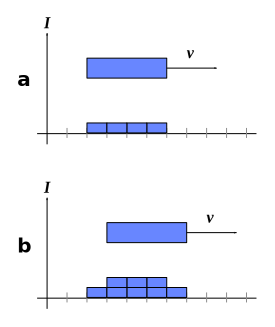
\includegraphics[width=8cm]{integration_blur.pdf}
\caption[Motion Blur Caused by Camera Integration]{
a) In this simplified, orthographic-projection camera, photosites integrate the scene intensity vertically ($I$) b) When the object moves at during the image exposure, the light from the object is distributed across multiple photosites, resulting in motion blur.
}
\label{fig:integration_blur}
\end{figure}

In a projective geometry imaging system, such as most cameras, blur from camera or object linear motion in any plane perpendicular to the optical axis appears as a linear \enquote*{smear} in the image x or y directions.
This \enquote*{smear} is known as a Point Spread Function (PSF), as it describes the spreading that occurs to the image of a perfect point source within the scene.
This is analogous to the impulse response of a frequency domain system; in this case the system is the optical apparatus, and the impulse is the point source in the scene.

Movement along the optical axis results in a radially varying PSF, while camera or object rotation creates a more complex PSF again.
In all cases, the degree of blur varies with the distance from the camera to the object moving.
For the sake of simplicity, in the experiments performed here we focus only on de-blurring linear motion blur induced through camera motion.

In order to de-blur light field data, it was necessary to quantitatively describe the way motion blur forms in a camera.
Specifically, it was necessary to derive an equation describing the way a motion blur PSF varied with respect to scene depth.
To do this, the homogeneous projective geometry equation was used;

\begin{equation}
\label{eq:camera_projection_unexpanded}
k \boldsymbol{x} = \boldsymbol{K} \left[~\boldsymbol{R}~|~\boldsymbol{t}~\right] \boldsymbol{X}
\end{equation}

\noindent
where $k$ is the homogeneous scaling constant, $\boldsymbol{x}$ is the image-space point location, $\boldsymbol{K}$ is the so-called \enquote*{camera intrinsic matrix} that accounts for camera distortions, $\boldsymbol{R}$ is the 3x3 camera rotation matrix,  $\boldsymbol{t}$ is the camera's 3x1 world-frame translation vector and $\boldsymbol{X}$ is the world-frame point location.

Expanding the matrix and vector terms, equation \ref{eq:camera_projection} is reached.

\begin{equation}
\label{eq:camera_projection}
k
\begin{bmatrix}
x \\
y \\
1 \\
\end{bmatrix}
=
\begin{bmatrix}
\alpha && s && u_0 \\
0 && \beta && v_0 \\
0 && 0 && 1 \\
\end{bmatrix}
\begin{bmatrix}
r_{11} && r_{12} && r_{13} && t_x \\
r_{21} && r_{22} && r_{23} && t_y \\
r_{31} && r_{32} && r_{33} && t_z \\
\end{bmatrix}
\begin{bmatrix}
X \\
Y \\
Z \\
1
\end{bmatrix}
\end{equation}

Here the intrinsic matrix $\alpha$ and $\beta$ terms are the camera focal length, scaled to be in units of x and y pixels respectively, $s$ is a shearing factor that describes the shear of the camera sensor (see Figure \ref{fig:intrinsic_shear}) and $u_0$ and $v_0$ are the x and y pixel locations of the optical axis of the camera.

\begin{figure}[h]
\centering

\includegraphics[width=4cm]{pixel_shear.pdf}
\caption[Camera intrinsic matrix shear term]{Camera intrinsic matrix shear term description, $s = \beta\tan(\theta)$. Figure from \cite{pollefeys2002visual}}
\label{fig:intrinsic_shear}
\end{figure}

Assuming the world frame coincides with the camera location and orientation, and assuming linear, horizontal camera motion at velocity $v_c$ meters per second with an exposure time of $t_e$ seconds, the blur width of a point source in the scene can be derived;

\begin{align}
w &= \left| x_1 - x_2 \right| \notag \\
&= \left| \left( \frac{\alpha + s + u_0}{Z} \right) X_1 - \left( \frac{\alpha + s + u_0}{Z} \right) X_2 \right| \notag \\
&= \left| \left( \frac{\alpha + s + u_0}{Z} \right) \left(\frac{- v_c t_e}{2}\right) - \left( \frac{\alpha + s + u_0}{Z} \right) \left(\frac{v_c t_e}{2}\right) \right| \notag \\
\label{eq:blur_width_full}
&= \left( \frac{\alpha + s + u_0}{Z} \right) v_c t_e
\end{align}

Finally, if we then assume square sensor pixels with no sensor skew, and an aligned optical axis, equation \ref{eq:blur_width_full} simplifies to

\begin{equation}
\label{eq:blur_width_simple}
w = \frac{f}{Z} v_c t_e
\end{equation}

\noindent
where $f$ is the focal length of the camera.
This equation describes the width of the linear motion blur created by a point source at depth $Z$ within the scene for a moving camera.
Note that the blur width is proportional with the camera focal length, velocity and exposure time, and inversely proportional with depth.
The inverse relation with scene depth correlates with the intuitive expectation; objects further away translate less in an image when the camera moves.
Equation \ref{eq:blur_width_simple} can be thought of as describing a 3D point spread function with $x$, $y$ and $Z$ as the dimensions.
This is shown visually in Figure \ref{fig:psf_3d}.


\begin{figure}[h]
\centering
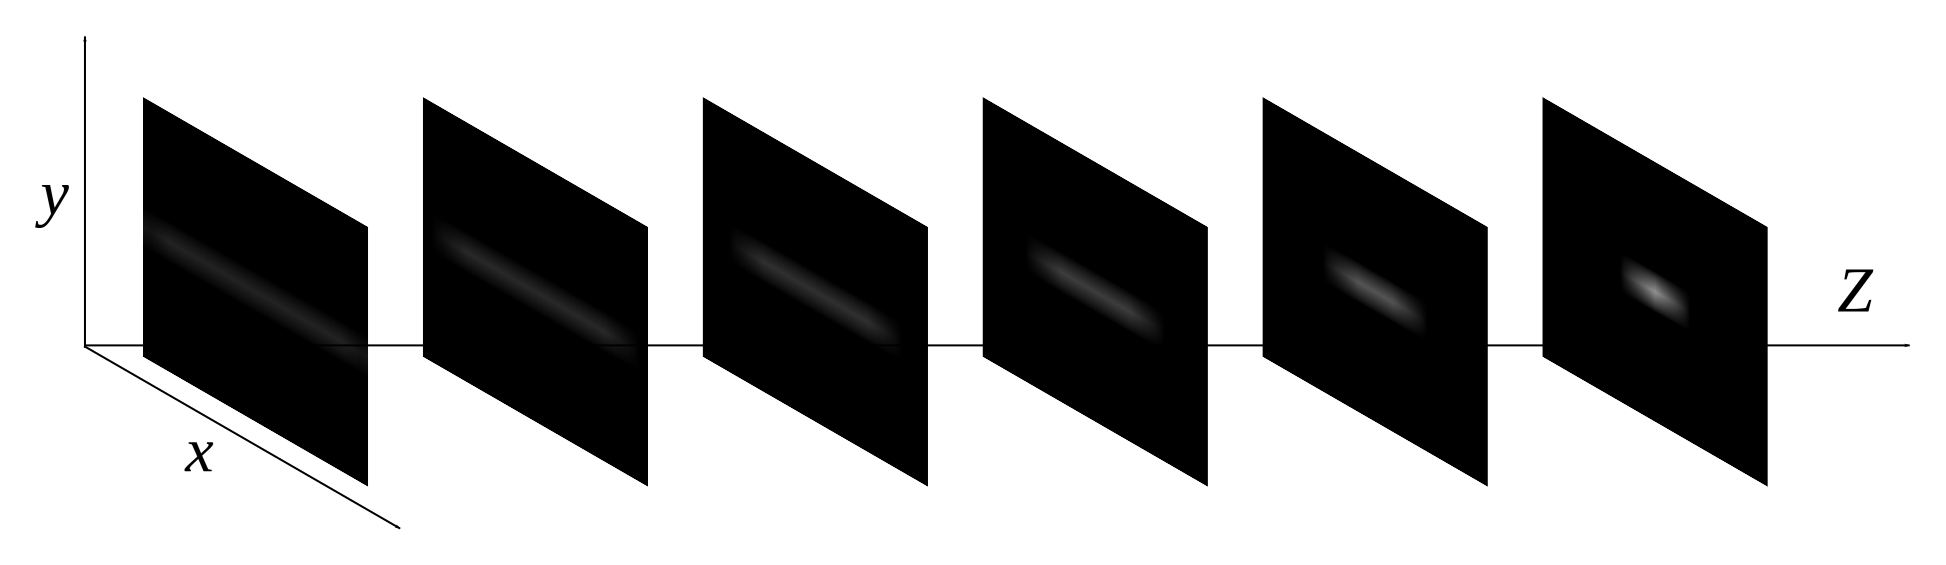
\includegraphics[width=\textwidth]{psf_3d.pdf}
\caption[Visualisation of a 3D Point Spread Function]{Visualisation of a 3D Linear Motion Point Spread Function, with $x$, $y$ and $Z$ as the dimensions}
\label{fig:psf_3d}
\end{figure}

Equation \ref{eq:blur_width_simple} was verified experimentally by taking several photos with a Lytro camera at a controlled velocity and measuring the blur width and depth of objects within the scene.
Only the central sub-aperture image from the light field was used for simplicity.
Figure \ref{fig:blur_vs_depth} shows the measured results along with the predicted curve.

\begin{figure}[h]
\centering
\includegraphics[width=\textwidth]{blur_vs_depth.pdf}
\caption[Edge Blur Width vs. Depth]{
Edge Blur Width vs. Depth - Measured and Predicted
}
\label{fig:blur_vs_depth}
\end{figure}

As can be seen, the equation matched the theoretical curve very closely, indicating that Equation \ref{eq:blur_width_simple} is a good fit for an individual sub-aperture image within a Lytro light field.
This shows that if the focal length, linear camera velocity and exposure time are known, and if a calibrated depth map can be recovered from the light field, it should be possible to de-blur all sub-aperture images from the light field image at all scene depths.
This is the basis for the light field de-blurring technique developed here.
As a final note, observe that the above analysis could also be applied to compute the 3D point spread function for a general camera trajectory, provided the trajectory (camera $\boldsymbol{R}$ and $\boldsymbol{t}$ at all times during the exposure) was known.
This possibility is discussed further in Chapter \ref{chap:results_and_discussion} (\nameref{chap:results_and_discussion}).


\section{Image De-blurring}
\label{sec:image_deblurring}

Knowledge of the way blur forms in a camera is pointless without a means to remove this blur.
There are several techniques used to remove the effects of motion and focal blur, the most common of which involve deconvolution.

As discussed in Section \ref{sec:motion_blur_formation}, motion blur is formed by camera or object movement during the camera exposure.
This is equivalent to convolution of a true image $f$ with the blur kernel or \enquote*{Point Spread Function} $g$.

\begin{equation}
\label{eq:spatial_blur_simple}
i(x) = f(x)~\textasteriskcentered~g(x)
\end{equation}

Writing this in the frequency domain, we get

\begin{equation}
\label{eq:frequency_blur_simple}
I(f) = F(f) \times G(f)
\end{equation}

\noindent
where $I$ is the observed image, $F$ is the original image and $G$ is the Fourier transform of the PSF, the so-called Optical Transfer Function (OTF).
Note that in the frequency domain, the convolution operator (\textasteriskcentered) is a simple element-wise multiplication and is therefore computationally fast.
This is the reason most image de-blurring techniques are performed in the frequency domain.

Supposing that the function $G$ can be found, it should theoretically be possible to recover the true image using

\begin{equation}
\label{eq:frequency_blur_inverse_simple}
F(f) = \frac{I(f)}{G(f)}
\end{equation}

\noindent
where element-wise division is used, and the inverse Fourier transform of $F$ is taken.
Unfortunately, in practice this is not possible for two reasons; firstly, $G$ will contain zeros that cause the values of $F$ to go to infinity.
Secondly, in practice the imaging system is subject to noise, indicated by $n$ (or $N$ in the frequency domain).
This can come in the form of Poisson shot noise, caused by the quantum nature of light, as well as device-specific detection noise.

\begin{equation}
\label{eq:frequency_blur_full}
I(f) = F(f) \times G(f) + N(f)
\end{equation}

These two factors mean that recovering the true image $f$ is not possible in practice.
Deconvolution de-blurring methods are an attempt to find a function $f'$ that estimates $f$ as accurately as possible, whilst being robust to the presence of additive noise.

De-convolution methods can be divided into several categories.
Linear deconvolution methods are most similar in operation to Equation \ref{eq:frequency_blur_inverse_simple}.
The most naive deconvolution is a regularised form of Equation \ref{eq:frequency_blur_inverse_simple}, where values in $F$ that would otherwise be infinite (due to zeros in $G$) are set to 0;

\begin{equation}
\label{eq:regularised_deconvolution}
F(f) = \begin{cases}
	\frac{I(f)}{G(f)},	& \left| H(f) \right| \ge \epsilon> 0 \\
	0					& \text{otherwise}
\end{cases}
\end{equation}

This is sometimes known as \enquote*{stabilised} deconvolution.
Note that regularised deconvolution does nothing to account for noise in the image, and will therefore \enquote*{amplify} the presence of noise in the recovered image $f'$.

Wiener filtering improves on this and is a general signal processing technique that attempts to recover an estimate of a signal in the presence of additive noise \cite{wiener1964extrapolation}.
Applied to image processing, Wiener deconvolution can be written as

\begin{equation}
\label{eq:wiener_filter}
F(f) = I(f) \left( \frac{G(f)^* \hat{I}(f)}{\left| G(f) \right|^2 \hat{I}(f) + \hat{N}(f) } \right)
\end{equation}

\noindent
where $\hat{I}$ and $\hat{N}$ are the mean spectral power densities of observed image $i$ and the noise $n$ respectively and $*$ denotes complex conjugation.
As can be seen, at frequencies with high noise, the Wiener filter suppresses the output, $F$ reducing the amplification of noise that regularised deconvolution suffers from.
Winer deconvolution has the drawback that the spectral content of the image and noise must be known, or estimated.

More complex convolution methods are framed in an iterative fashion.
These methods iteratively solve the minimisation of some cost function.
This cost function can be defined in a least-squares framework \cite{ng99anew} or as an expectation-maximisation problem, as is the case with the well known Richardson-Lucy deconvolution method \cite{richarson1972bayesian}.
This method seeks to maximise the probability of observing the image $I$ if the true image is some other trial image.

Finally, blind deconvolution methods are a collection of more recent techniques where no information about the PSF needs to be supplied \cite{bell1995information, ayers1988iterative}.
In these methods, an estimate of the original image is made, then convoled with a theoretical PSF.
This is compared with the observed image and corrections made to both the PSF and original image estimates.
The process then repeats iteratively until some stopping criterion is met.
These methods have the obvious advantage that they operate without the prior PSF.

In our experiments we apply Richardson-Lucy deconvolution to a light field image, using the depth map to vary the PSF for different parts of the scene.
Richardson-Lucy deconvolution was selected due to it's computational simplicity and robust performance in the presence of noise, however any deconvolution method could be used in it's place.
We compare the results of our depth-aware deconvolution technique with those of Regularised, Blind and 2D Richardson-Lucy deconvolution to demonstrate the improvement that using a depth-aware PSF brings.

\section{Light Field Depth Estimation}
\label{sec:light_field_depth_estimation}

As shown in section \ref{sec:motion_blur_formation}, de-blurring at all scene depths requires a depth map calibrated to be in metric units such as meters.
It was found that the Lytro firmware and/or desktop software computes a low-quality depth map from the Lytro Light Field images, returning integer depth values in an arbitrary unit.
These depth maps are located within the Lytro image storage database and are contained in Lytro image files with the name \enquote*{dm.lfp}.
The \enquote*{lfpsplitter} tool \cite{patel2013lfptools} was used to extract this data into a single-column text file format, after which Matlab was used to reshape this data into a depth map.
To correctly re-shape the data, it had to be read in standard raster order (left to right, top to bottom), with an expected size of 330x330.
In the resulting depth maps, lower (darker) values indicate objects closer to the camera.

Further research and analysis is needed to more fully quantify the Lytro depth response function, however an initial investigation was performed using several Lytro images.
Sample points from within the Lytro depth maps were compared with metric depth estimates for a range of scenes, with the scene depth ranging up to \nicetilde2.5 meters.
Our initial analysis showed that after the rejection of outliers, the Lytro depth response \enquote*{$D$} was a linear function with metric object depth \enquote*{$Z$}, however the specific linear function varied as the overall scene depth range changed.
For example, scenes with an overall depth range less than 0.5m were found to be a good fit ($R^2 = 0.69$) with the linear function $Z(D) = 0.0291 D + 0.2114$, while scenes with a depth range of 0.5-2.5m were a good fit ($R^2 = 0.7$) with the function $Z(D) = 0.1503 D + 0.781$.
More data is needed to derive a continuous function $D \Rightarrow Z$, however for simplicity the piecewise mapping described here was used in our experiments.
Figure \ref{fig:depth_real_world_vs_lytro_response} shows these results in graph format.

Thus, if prior information is available about the overall depth range of the scene ($\hat{Z}$), the Lytro depth map data can be calibrated to metric units;

\begin{equation}
\label{eq:lytro_dm_to_metric}
Z(D, \hat{Z}) = \begin{cases}
	0.0291 D + 0.2114, & \hat{Z} < 0.5m. \\
	0.1503 D + 0.781, & 0.5 \leq \hat{Z} < 2.5m. \\
\end{cases}
\end{equation}

\noindent
where $\hat{Z}$ is the \emph{a-priori} rough scene depth estimate.
Insufficient data was collected for scenes with depth beyond 2.5 meters to characterise the depth response in those regions.

It was found experimentally that the Lytro-generated depth maps have a minimum recoverable depth range of \nicetilde5cm and that the presence of glare prevents accurate depth estimation (see Figure \ref{fig:ruler_glare_min_dist}).
Furthermore, it was found that the presence of motion blur or lack of scene structure reduced the quality of the depth map (see Figures \ref{fig:depth_lack_of_structure} and \ref{fig:blur_corrupts_depth}).
The reduction in quality due to glare is expected due to the lambertian scene assumption made in many light field computational photography algorithms \cite{bishop2009light, liang2011light, baker2003shape} and the reduction in quality due to motion blur or lack of structure suggests the Lytro software is using a dense correlation based depth estimation method.

\begin{figure}[p]
\centering
\includegraphics[width=\textwidth]{depth_real_world_vs_lytro_response.pdf}
\caption[Lytro depth response vs. metric depth]{
Lytro depth response vs. metric depth.
The data has been binned into two categories based on overall scene depth range.
}
\label{fig:depth_real_world_vs_lytro_response}
\end{figure}

\begin{figure}[p]
\centering
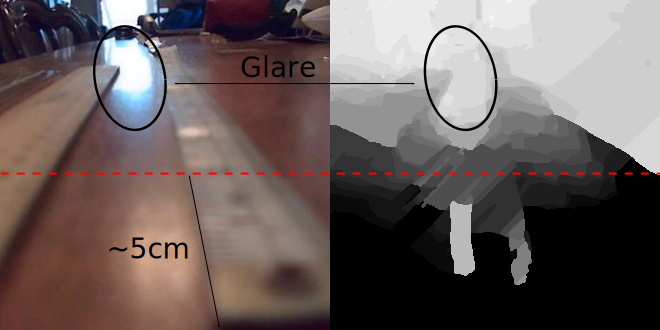
\includegraphics[width=\textwidth]{ruler_glare_min_dist.pdf}
\caption[Minimum depth map distance and the effect of glare]{
An example light field image, and the Lytro depth map response, normalised to the range [0, 1] for display.
Darker values are closer to the camera.
Note the lack of depth data where glare is present, and below Z = 5cm.
}
\label{fig:ruler_glare_min_dist}
\end{figure}

\begin{figure}
\centering
\includegraphics[width=\textwidth]{blur_corrupts_depth.png}
\caption[Motion Blur Corrupts Lytro Depth Estimation]{
The same scene photographed three times with the Lytro camera, with progressively more motion blur.
Note the reduction in the quality and consistency of the depth response.
Depth maps have been normalised to the range [0, 1] for display, and darker values are closer to the camera.
}
\label{fig:blur_corrupts_depth}
\end{figure}

These findings suggested that if rough knowledge of the scene depth could be obtained, it would possible to calibrate the Lytro depth maps into metric units.
We suggest that in a real-world application, an infra-red/ultrasound based focal length sensor (as found on many commercial cameras) could be used for this purpose.
Alternately, user-supplied a-priori knowledge of a robotic operating environment, or a user-selected \enquote*{scene} setting on a commercial camera (e.g. outdoors, indoors, portrait etc.) could be used here.

Finally, in addition to using the Lytro software depth maps, the possibility of using other depth estimation methods was explored.
In particular, the \enquote*{Depth from Combining Defocus and Correspondence} method by Tao et al. \cite{tao2013depth} was tested.
Using the supplied Matlab source code \cite{tao2013depthwebsite}, depth maps were found to be extremely noisy and completely unusable (see Figure \ref{fig:defocus_correspondence_depth}).
It is possible this was due to their code being tuned specifically for their Lytro camera, however due to discovering the more readily available Lytro depth data, this possibility was not explored further.

\begin{figure}[p]
\centering
\includegraphics[width=\textwidth]{depth_lack_of_structure.png}
\caption[Lack of Scene Structure Corrupts Lytro Depth Estimation]{
An example light field image and the Lytro depth response, normalised to the range [0, 1] for display.
Darker values are closer to the camera.
Note the lack of clear structure in some parts of the image (e.g. on the stuffed toy's face and body, and in the background) results in large regions without depth variation, despite the presence of metric depth change.
}
\label{fig:depth_lack_of_structure}
\end{figure}

\begin{figure}[p]
\centering
\includegraphics[width=7cm]{defocus_correspondence_depth.png}
\caption[Depth Map from combining Defocus and Correspondence]{
An example depth map result from using Defocus and Correspondence by Tao et al. \cite{tao2013depthwebsite}.
The input light field is the same as in Figure \ref{fig:depth_lack_of_structure}.
Darker values are supposedly closer to the camera, although the depth map does not match the real world depths.
}
\label{fig:defocus_correspondence_depth}
\end{figure}


In summary, it was found that if a rough scene depth estimate is known, the Lytro depth maps could be calibrated to metric units.
This was the final element needed to enable depth-aware deconvolution of light field images, as it allowed the blur at every point in the light field to be determined, using Equation \ref{eq:blur_width_simple}.
